\subsection{SciCode}
{{\footnotesize
\noindent SciCode is a scientist-curated coding benchmark with 338 subproblems derived from 80
real research tasks across 16 scientific subfields, evaluating models on knowledge recall, 
reasoning, and code synthesis for scientific computing tasks.


\begin{description}[labelwidth=4cm, labelsep=1em, leftmargin=4cm, itemsep=0.1em, parsep=0em]
  \item[date:] 2024-07-18
  \item[version:] 1
  \item[last\_updated:] 2024-07-18
  \item[expired:] false
  \item[valid:] yes
  \item[valid\_date:] 2024-07-18
  \item[url:] \href{https://arxiv.org/abs/2407.13168}{https://arxiv.org/abs/2407.13168}
  \item[doi:] 10.48550/arXiv.2407.13168
  \item[domain:] Scientific Programming
  \item[focus:] Scientific code generation and problem solving
  \item[keywords:]
    - code synthesis
    - scientific computing
    - programming benchmark
  \item[licensing:] unknown
  \item[task\_types:]
    - Coding
  \item[ai\_capability\_measured:]
    - Program synthesis, scientific computing
  \item[metrics:]
    - Solve rate (\%)
  \item[models:]
    - Claude3.5-Sonnet
  \item[ml\_motif:]
    - Coding
  \item[type:] Benchmark
  \item[ml\_task:]
    - Supervised Learning
  \item[solutions:] unknown
  \item[notes:] Good
  \item[contact.name:] Minyang Tian
  \item[contact.email:] mtian8@illinois.edu
  \item[datasets.links.name:] unknown
  \item[datasets.links.url:] \href{unknown}{unknown}
  \item[results.links.name:] unknown
  \item[results.links.url:] \href{unknown}{unknown}
  \item[fair.reproducible:] True
  \item[fair.benchmark\_ready:] True
  \item[id:] scicode
  \item[Citations:] \cite{tian2024scicoderesearchcodingbenchmark}
\end{description}

{\bf Ratings:} ~ \\

\begin{tabular}{p{0.15\textwidth} p{0.07\textwidth} p{0.7\textwidth}}
\hline
Rating & Value & Reason \\
\hline
dataset & 0 & Paper and website had no link to any dataset. It may still exist somewhere
 \\
documentation & 4 & Paper containing all needed info except for evlauation criteria
 \\
metrics & 2 & Metrics stated, but method of grading is not specified
 \\
reference\_solution & 1 & Models presented with scores, but none are open or list constraints
 \\
software & 5 & Code to run exists on github repo
 \\
specification & 4.5 & Expected outputs and broad types of inputs stated. Few details on output grading. No HW constraints.
 \\
\hline
\end{tabular}

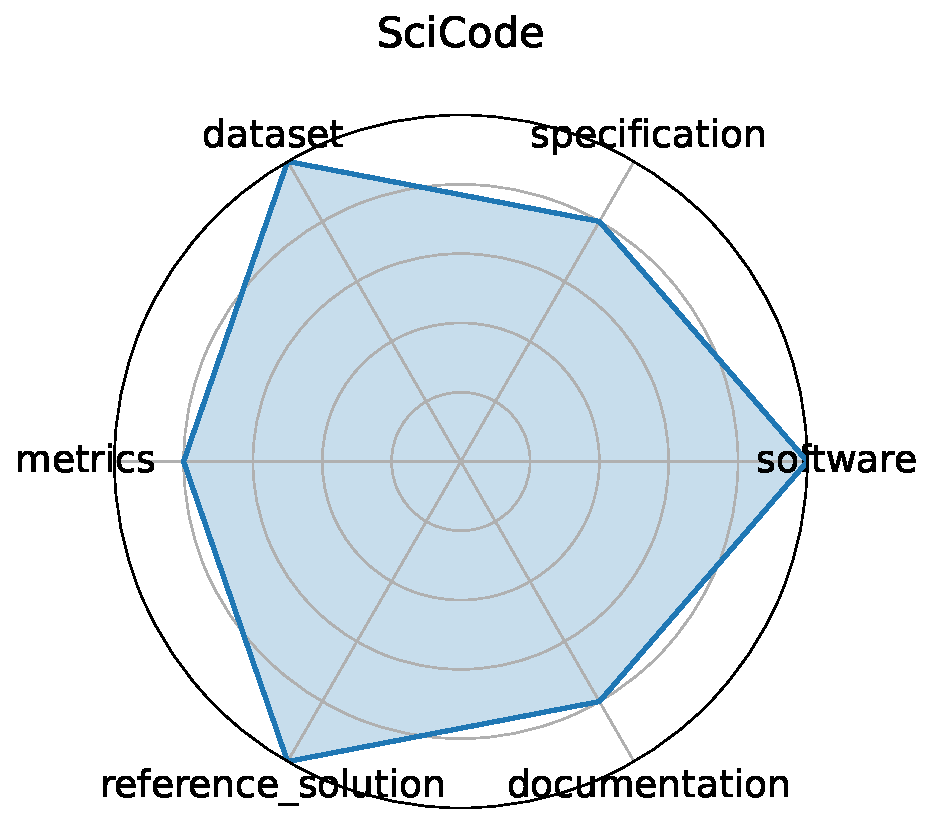
\includegraphics[width=0.2\textwidth]{scicode_radar.pdf}
}}
\clearpage